%%%%%%%%%%%%%%%%%%%%%%%%%%%%%%%%%%%%%%%%%
% Stylish Article
% LaTeX Template
% Version 2.2 (2020-10-22)
%
% This template has been downloaded from:
% http://www.LaTeXTemplates.com
%
% Original template author:
% Mathias Legrand (legrand.mathias@gmail.com) 
% With extensive modifications by:
% Vel (vel@latextemplates.com)
% Christoph Werries (cwerries@uni-osnabrueck.de)
%
% License for template:
% CC BY-NC-SA 3.0 (http://creativecommons.org/licenses/by-nc-sa/3.0/)
%
%%%%%%%%%%%%%%%%%%%%%%%%%%%%%%%%%%%%%%%%%

%----------------------------------------------------------------------------------------
%	PACKAGES AND OTHER DOCUMENT CONFIGURATIONS
%----------------------------------------------------------------------------------------
\documentclass[10pt]{SelfArx} % Document font size and no equations flushed left

\usepackage[english]{babel} % Specify a different language here - english by default

\usepackage{lipsum} % Required to insert dummy text. To be removed otherwise

\usepackage[nolist]{acronym}	% [nolist]: Acronym list should not be print out.

\usepackage{listings}	% Required to insert lstlisting environment for code.

\usepackage{makecell}	% For manual line breaks in tables

\usepackage{caption}
\usepackage{subcaption}	% Needed for subfigures

\usepackage{longtable}

\usepackage{tikz}

\makeatletter
\newcommand\mycircle{\@currsize\tikz[baseline=(n.210),inner sep=0pt]%
  \node[line width=0.1em, circle,minimum size=0.7\baselineskip,draw](n){};%
  }

%\myfillcircle[zufüllender Winkel in Grad]
\newcommand\myfillcircle[1][360]{%
  \@currsize\tikz[baseline=(n.210),inner sep=0pt]%
    \fill(0,0)%
      node[line width=0.1em, circle,minimum size=0.7\baselineskip,draw](n){}%
      --+(0,0.35\baselineskip)%
      arc[start angle=90,end angle=90+#1, radius=0.35\baselineskip];%
}

%----------------------------------------------------------------------------------------
%	COLUMNS
%----------------------------------------------------------------------------------------
\setlength{\columnsep}{0.55cm} % Distance between the two columns of text
\setlength{\fboxrule}{0.75pt} % Width of the border around the abstract

%----------------------------------------------------------------------------------------
%	COLORS
%----------------------------------------------------------------------------------------
\definecolor{color1}{RGB}{172,06,52} % Corporate Design Colour of University of Osnabrueck
\definecolor{color2}{RGB}{207,208,209} % Corporate Design Colour of University of Osnabrueck
\definecolor{color3}{RGB}{251,185,0} % Corporate Design Colour of University of Osnabrueck
\definecolor{codegreen}{rgb}{0,0.6,0}
\definecolor{codegray}{rgb}{0.5,0.5,0.5}
\definecolor{codepurple}{rgb}{0.58,0,0.82}
\definecolor{backcolour}{rgb}{0.95,0.95,0.92}

%----------------------------------------------------------------------------------------
%	LISTING STYLE
%----------------------------------------------------------------------------------------
\lstdefinestyle{mystyle}{
    backgroundcolor=\color{backcolour},   
    commentstyle=\color{codegreen},
    keywordstyle=\color{magenta},
    numberstyle=\tiny\color{codegray},
    stringstyle=\color{codepurple},
    basicstyle=\ttfamily\footnotesize,
    breakatwhitespace=false,         
    breaklines=true,                 
    captionpos=b,                    
    keepspaces=true,                 
    numbers=left,                    
    numbersep=5pt,                  
    showspaces=false,                
    showstringspaces=false,
    showtabs=false,
    tabsize=2
}
\lstset{style=mystyle}

%----------------------------------------------------------------------------------------
%	HYPERLINKS
%----------------------------------------------------------------------------------------
\usepackage{hyperref} % Required for hyperlinks
\hypersetup{
	hidelinks,
	colorlinks=true,
	breaklinks=true,
	urlcolor=color3,
	citecolor=color1,
	linkcolor=color1,
	bookmarksopen=false,
	pdftitle={Title},
	pdfauthor={Author}
}

\usepackage{apacite}
\AtBeginDocument{\urlstyle{APACsame}}

%----------------------------------------------------------------------------------------
%	ARTICLE INFORMATION
%----------------------------------------------------------------------------------------
\JournalInfo{
\includegraphics[width=0.3\linewidth]{figures/logo_uni}}
\Archive{} %!!NEEDED, otherwise \tableofcontent error, is for Additional notes below university logo (e.g. copyright, DOI, review/research article)

\PaperTitle{Happywhale - Automated Marine Animal Recognition}

\Authors{Louis Kapp, Felix Hammer}

\Keywords{Triplet loss, Nature Conservation, Machine Learning} 
\newcommand{\keywordname}{Keywords}

%----------------------------------------------------------------------------------------
%	ABSTRACT
%----------------------------------------------------------------------------------------
\Abstract{As the urgency of nature conservation rises daily, see it as our responsibility to support this endeavor by means of technology. The Kaggle Happywhale challenge, with the goal of individual whale recognition, provides the perfect opportunity to this using machine learning. In this paper, we investigate the usefulness of combining Softmax classification with a semi hard triplet-loss approach. We also test performance of several Convolutional Neural Network architectures. Our test findings conclude that InceptionV3 is the best performing architecture, although combining Softmax and Triplet loss is not a useful approach (in spite reduced convergence time). It turns out that our "lazy" approach is not sufficient for obtaining good results. A likely cause is our usage of semi-hard triplets, while the dataset contains many hard triplets.}

%----------------------------------------------------------------------------------------
%   BEGIN DOCUMENT
%----------------------------------------------------------------------------------------
\begin{document}
\maketitle

%\tableofcontents
\thispagestyle{empty} % Removes page numbering from the first page

%----------------------------------------------------------------------------------------
%	ARTICLE CONTENTS
%----------------------------------------------------------------------------------------
\section{Introduction}
\addcontentsline{toc}{section}{Introduction}
\label{sec:intro}

As climate change and environmental pollution intensify, nature conservation becomes increasingly important. A part of nature conservation is also the study of animal behavior, migration routes and population density, to better understand the problem and obstacles certain species are facing, so we can tackle and prevent these problems to the best of our abilities. To do this, we must be able to differentiate between individuals of a species. In humans, this is easily done by face or fingerprint recognition. But what about animals? \\
To date researchers manually differentiate them by the shape and markings on their tails, dorsal fins, heads and other body parts. This is time consuming and difficult work, since it takes the eye of a good researcher and much time to identify, match or tell individual animals apart. \\ Hence the question arises: When we can use automated identification for humans, is there a similar approach possible for animals? \\
The recent advances in facial recognition were mostly commercially motivated. Photo identification for animals seems like a less lucrative endeavour which moves it out of the research limelight. However, a technique like this could simplify the analysis of wildlife 
and therefore nature conservation significantly.\\
This is why we decided to take on the Kaggle Happywhale challenge \cite{kaggle}. This goal of this challenge is to train a machine learning model to identify whales and dolphins individuals. The competitions winning model will be used on happywhale.com \cite{happywhaledotcom}, a research collaboration platform which aims at increasing global understanding and caring for marine animals. \\ 
We want to use this challenge to look for relevantly easy approaches that could be implemented by conservation organizations to automatically detect individuals on their data-sets as well.

\section{Kaggle Happywhale Challenge}
\addcontentsline{toc}{section}{Kaggle Happywhale Challenge}
\label{sec:kagglechallenge}

In the following chapter, we are explaining the Kaggle Happywhale challenge. This includes goal-setting and a comprehensive analysis of the dataset.

\subsection{Goal}
The Happywhale challenge is a research prediction competition, open to everybody with a Kaggle account. It's goal is to build a machine learning model which can reliably recognize individual whales and dolphins. The model should also be able to classify individuals it has never seen before as "new".
Such a model would save experts, who - up until now - have to analyse the images manually, a tremendous amount of work.


\subsection{Data}
The data \cite{kaggle} to be used for this challenge is split in to training and testing data. The training data consists of 51 thousand JPEG images of whales and dolphins. The training images are labeled with the according species and a unique individual identification string. The testing data consist of 28 unlabeled images containing some new whales and dolphins which are not present in the training data.\\
In total there are about 15 thousand different individuals and 30 different species. This data was manually curated by researchers from all over the world.

\begin{figure}[ht] 
        \centering 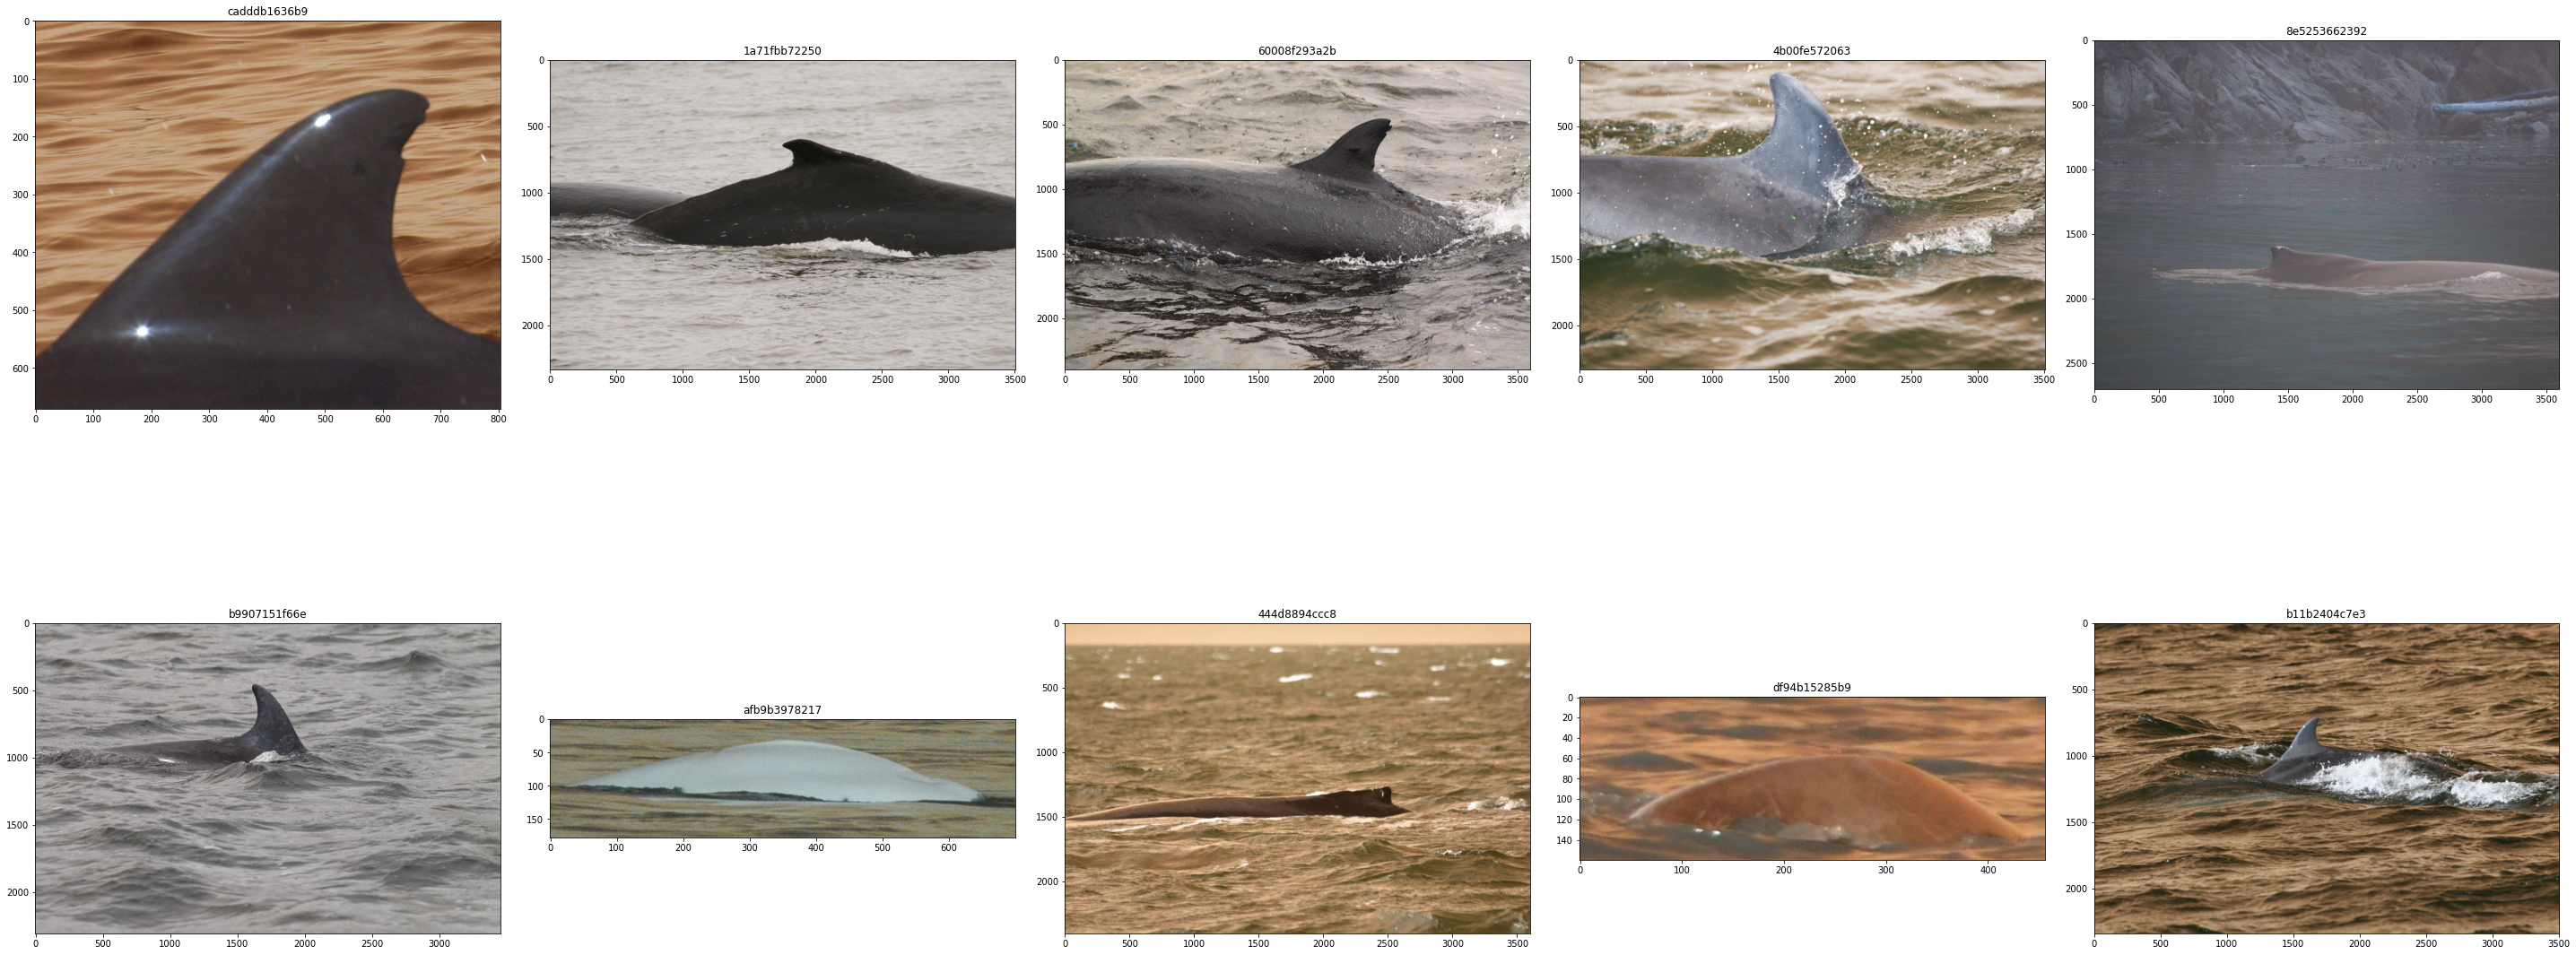
\includegraphics[width=1\columnwidth]{figures/original_images.png}
        \caption{\label{fig:original_images} Typical images from the data set.}
\end{figure}

\noindent With a median image shape of approximately (3000,1500), most images have high resolution. This makes unique patterns and markings of each individual identifiable by a neural network, even though most images only contain small parts of the marine animals such as dorsal fins and parts of the backs. \\
Some further analysis shows that 59\% of all individuals have only one image of themselves. They make out 18\% of all images in the data set.
5\% of all individuals have at least 10 images of themselves. These are 47\% of all images in the data set. \\
This is a large unbalance in number of images per individual and will make training of the network much harder.
\section{Model selection}
\addcontentsline{toc}{section}{Model selection}
\label{sec:model_selection}

At first glance, one could think that the problems like the Happywhale challenge are generic multi-class classification task. This would mean that the model should be able to classify an input image of an individual correctly as just this individual. For tasks like this, the default approach is the following: \\
Feed the input image to some Convolutional Neural Network (CNN) architecture which outputs an embedding of this image. This embedding can then be flattened and fed into a Dense Layer which will output the predicted class. \cite{CNN-Courseware}

\begin{figure}[ht] 
        \centering 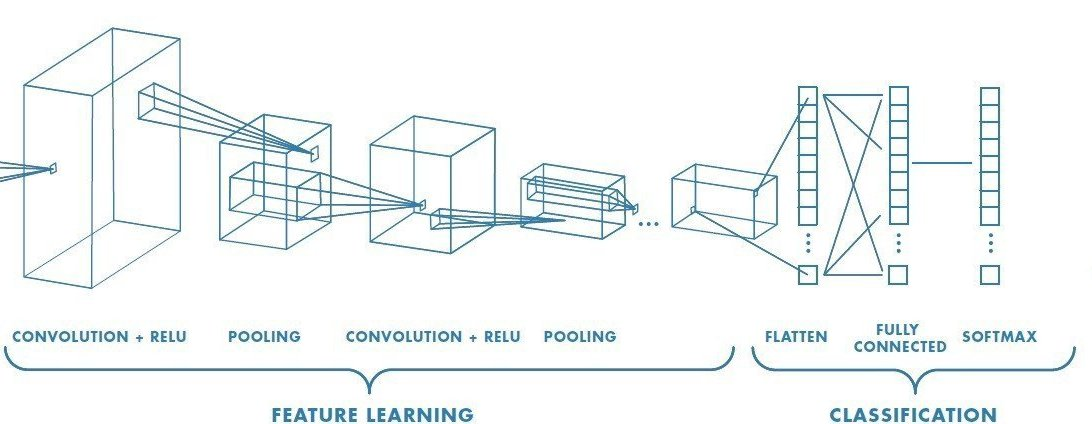
\includegraphics[width=1\columnwidth]{figures/cnn.jpeg}
        \caption{\label{fig:cnn_architecture_img} Vanilla image classification \protect\cite{cnn_architecture_img}.}
\end{figure}

\subsection{CNN architecture} \label{subsec:cnn}
As a first step of model selection we compare popular CNN architectures that we want to test. It is often a good idea to bet on architectures which already solidified their position on the grandstand of the machine learning domain of interest. Therefore we had a look at the most implemented models for image classification tasks. \\
Looking at this list we decide for a Residual Neural Network (ResNet), a Densely Connected Neural Network (DenseNet), an EfficientNet and an InceptionNet. \cite{paperswithcode}
All of these networks are notorious for being capable to classify images with very high accuracy while being somewhat computationally efficient (at least compared to other machine learning approaches). \\ 
Additionally, there are countless pre-trained models with easy access points available for these architectures. Especially the models pretrained on ImageNet \cite{deng2009imagenet}, one of the world's largest labeled image databases, are extremely powerful for image classification tasks and therefore of great interest to us. \\
We decided to try out the following architectures with pre-trained weights from ImageNet: ResNet50, ResNet50V2, DenseNet101, EfficientNet and InceptionNetV3. We also trained ResNet50 ourselves. More about that can be read in \hyperref[sec:softmax-model]{Softmax Model}.

\subsection{Softmax activation}
The activation function of the last Dense Layer in this pipeline is usually a Softmax function \shortcite{Training-Courseware}, which computes a probability distribution \(\sigma\) over the image membership for each class \(K\).
\[ \sigma(z_i) = \frac{e^{z_{i}}}{\sum_{j=1}^K e^{z_{j}}} \ \ \ for\ i=1, \dots, K \ \ \ \text{and} \ \ \ (z_1, ..., z_K) \in \mathbb{R}^K \]
\(K\) is determined by the constant number of neurons in the final Dense Layer.
Unfortunately, we are working with a dynamically changing number of classes - we do not know every individual whale in the ocean (let alone having images of them). \\
For now, this eliminates the Softmax activation function as a suitable approach to our task. \\

\subsection{Triplet loss}
Luckily, the domain of metric learning offers us an alternative approach which is more suitable for our problem: Triplet loss - originally presented in the FaceNet \cite{Schroff_2015} paper. \\
The goal of triplet loss is to learn an embedding space in which similar sample pairs stay close together and dissimilar ones are far apart. It does this by computing a distance between an anchor image \(a\) and a positive sample \(p\), as well as between \(a\) and a negative sample \(n\). \(a\) and \(p\) are different images of the same individual, while \(n\) is an image of a different individual.

\begin{figure}[ht] 
        \centering 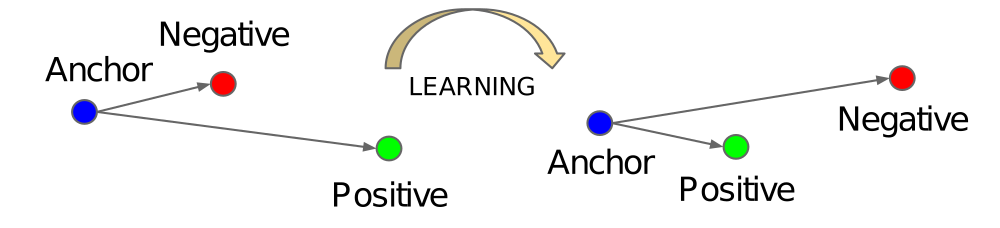
\includegraphics[width=1\columnwidth]{figures/triplet_loss.png}
        \caption{\label{fig:triplet_loss_img} Triplet loss visualized \protect\cite{Schroff_2015}.}
\end{figure}

\noindent The learning goal is then to minimize the distance between \(a\) and \(p\) and maximize the distance between \(a\) and \(n\) at the same time \cite{weng2021contrastive}. Triplet Loss for some triplet \((a,p,n)\) in the embedding space is defined as:
\[ \mathcal{L}_\text{triplet} = \max\left(0,d(a,p)-d(a,n) + \epsilon\right) \]
where \(d\) denotes the L2 norm (calculated from the euclidean distance between the embeddings) and the margin parameter \(\epsilon\) denotes the minimum offset between distances of \(d(a,n)\) and \(d(a,p)\). This prevents the the network of gaming the function and circumventing its actual intention. If there was no \(\epsilon\), the network could just map the complete data set onto the same point in the embedding. This would cause all distances and the loss to be 0. The margin ensures, that in this case, the loss would still be positive. \cite{hav4ik2021deepmetriclearning}\\

\subsubsection{Triplet Mining} \label{subsec:mining}
Of course, triplet loss is far from being a perfect method of choice as well. One of it's main limitations is that during one comparison only one negative example \(n\) is compared with the anchor \(a\). The disregard of all other \(n\) could lead to an embedding space where some dissimilar pairs are still in close proximity to each other - just because they were not compared against each other. \cite{Sohn_2016} \\
This is why, in order to train a triplet loss model successfully, one has to pay close attention to the composition of each triplet. If we want the model to learn something we should pick an \(n\) that is not obviously a different individual than \(a\). \\

\noindent To do this, we could choose a challenging \(n\) that is closer to the \(a\) than the positive sample \(p\).
\[ d(a,n) < d(a,p) \]
This is called \textit{hard triplet mining}. In theory, it should guarantee optimal learning success. However, it is prone to get stuck in local minima and the samples are rather hard to select from our data set. \\

\noindent An approach which tries to solve this is \textit{semi-hard triplet mining}. Here the triplets are chosen in a way, that \(n\) is not closer to \(a\) than \(p\), but the function still has a positive loss.
\[ d(a,p) < d(a,n) < d(a,p) + \epsilon \]
The distance between \(a\) and \(n\) is still in the range of margin \(\epsilon\). This way, the model can still learn but is more unlikely to end up in local minima. \\

\begin{figure}[ht] 
        \centering 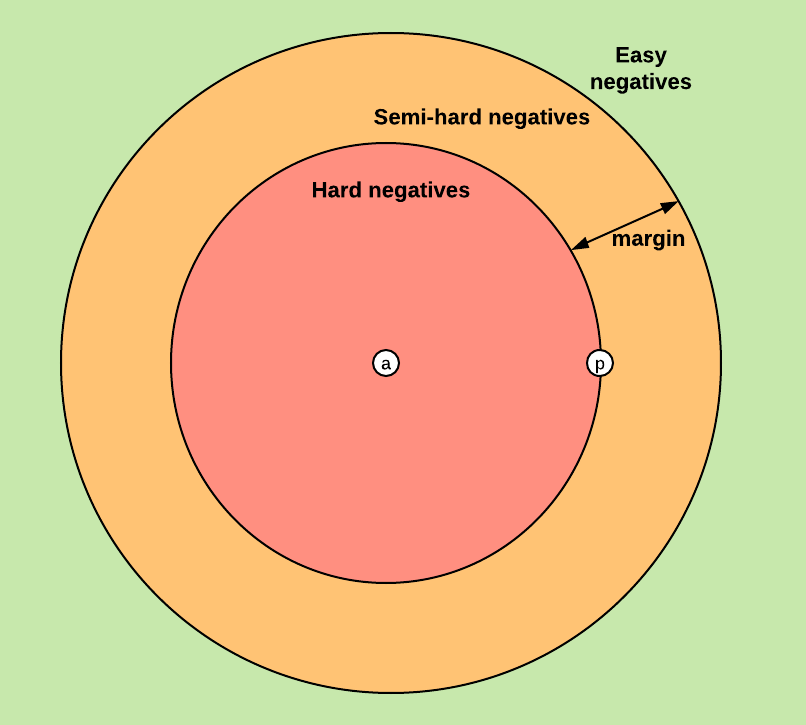
\includegraphics[width=1\columnwidth]{figures/triplet_mining.png}
        \caption{\label{fig:quellemussrein}Different kind of Negatives visualised \protect\cite{moindrot}.}
\end{figure}


\noindent We need to specify the triplet sampling process even further by choosing between \textit{offline} and \textit{online} triplet mining. \\
With \textit{offline mining}, the triplets are generated at the beginning of each epoch. The embeddings are computed on the training set and then only (semi-) hard triplets are selected. This technique is rather inefficient because we need to do a full pass on the training set for each epoch and update the triplets. \\
Doing \textit{online mining}, samples are produced for each batch of inputs. Within a batch of \(B\) examples we can find a maximum of \(B^3\) triplets. Many of these triplets are not of shape \((a,p,n)\) and are therefore not valid. Still, it does not require updating all samples offline and more samples are created for a single batch. This makes the approach way more efficient \cite{moindrot}.

\subsubsection{Shortcomings}
There still remain problems with the triplet loss function and contrastive learning approaches in general. \\
It is hard to guarantee that embeddings of the same individual will be pulled together in euclidean space (expansion problem). In addition, there is the so called sampling issue \cite{hav4ik2021deepmetriclearning}: Online triplet mining is hard to implement for very unbalanced data sets like our Happywhale data set. \\
There are modern alternatives to triplet loss such as Cos- and ArcFace, which are based on angular distance and margin. They (partially) solve the above problems but we nevertheless wanted to try out vanilla triplet loss and see how far we will come with this approach. Since our paper should also be of some educational value and explain the concepts well to other students, triplet loss is also more suitable because it is less advanced and needs fewer prerequisites to understand. \\
Because of the mentioned advantages in \hyperref[subsec:mining]{Triplet mining}, we also decided to implement online semi-hard triplet mining. \\
There is still one disadvantage of triplet loss which we did not talk about up until now: Evaluation of training progress is computationally expensive. As we want to evaluate the usefulness of the different \hyperref[subsec:cnn]{CNN architectures}, we need to compute an evaluation metric (i.e. accuracy) on the validation set after each training epoch. To do this, the embedding of every image from the validation set needs to be compared to all embeddings of the training set. This means there have to be many point-wise distance calculations in a high dimensional euclidean space calculated. To be specific, we need to do $37598 *  4177$ computations in a $256$-dimensional embedding space for each epoch. Furthermore, the convergence time for triplet loss models is said to be rather high. \\
Doing this for more multiple hyperparameter settings for each architecture is not feasible with our computational resources. Is there a cheaper workaround?

\subsection{Combining Softmax and Triplet Loss}
We already found out that the Softmax activation function is not useful for our final model but maybe we could still utilize it for some architecture comparison. Computing accuracy of a Softmax based model is a breeze compared to models based on contrastive loss. \\
We can imagine that an architecture that performs well over a finite-class classification task using Softmax is also likely to perform well for a classification problem with a dynamical number of classes like Happywhale. So why not try this out? \\
Our approach will now look like the this: \\
We will train the said models with a fixed size Softmax Dense layer at the end on the different (fixed) whale species. During this training process, we evaluate their performance on the validation set, taking accuracy and convergence speed into account. After training is finished, we compare their performance on the test set and select the most robust and promising architecture for our final triplet loss model.\\

\noindent The final model will essentially be a Siamese Network which is composed of 2 identical CNN architectures that share their weights. The according inputs are the sample pairs \((a,p)\) and \((a,n)\) which are then projected into the embedding space. As explained earlier, the triplet loss then should ensure reasonable euclidean distances between the embedding pairs.

\section{Hypotheses}
\addcontentsline{toc}{section}{Hypotheses}
\label{sec:hypotheses}

Knowing all this, we can motivate the following hypotheses that we want to investigate further:

\begin{enumerate}
    \item Is a "lazy" approach of just using prebuild \& pretrained architectures and preconfigured loss functions sufficient enough to produce significant results in individual classification?
    \item Is Softmax classification training success a useful indicator for triplet loss training success? To be specific: Does the best performing CNN architecture under Softmax also show best performance of under triplet loss?
    \item Can you reduce triplet loss training time with network weights pretrained on Softmax classification?
\end{enumerate}
\section{Data Pipeline}
\addcontentsline{toc}{section}{Data Pipeline}
\label{sec:data-pipeline}

\subsection{Preprocessing}
We apply several preprocessing steps to get the data into an optimal shape for our model. We also create One-hot labels.

\subsubsection{Normalization}
Normalization ensures that all images have same format.\\
One of the first steps is downsizing the images. Although our mostly high resolution pictures allow to see patterns and unique marks of the whales in great detail, we have to downsize the images enough that our memory can handle it. It is also useful to have every image in the same quadratic shape. We chose the shape (224, 224) since it is little enough to not run into memory constraints but still large enough for the model to recognize some details. The pretrained ImageNet-models also use this input size. The automatic interpolation of Tensorflow ensures that the images still look somewhat natural and not too distorted. \\
We also converted the pixel values from integers to floats to make sure that Tensorflow can work with them. The float values were fixed between -1 and 1.

\subsubsection{Foreground Extraction}
Since the images often contain much ocean in the background and the model should definitely not take this as feature, we thought it would be a good idea to crop the background such that only the whale on white background is in the image.\\
We mainly used preexisting algorithms from the Kaggle Humpback Whale challenge \cite{kapse} for this. Unfortunately, large parts of whales were cropped in many images. \\

\begin{figure}[ht] 
        \centering 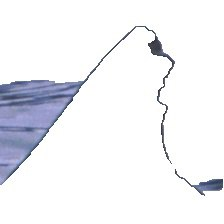
\includegraphics[width=0.7\columnwidth]{figures/whack_foreground_extraction.jpg}
        \caption{\label{fig:fe} Failed foreground extraction.}
\end{figure}

\noindent This is why we decided not to include this preprocessing step in our pipeline.

\subsubsection{Data Augmentation}
Data Augmentation has the goal of increasing the size of the data set. \\
This is especially useful for obtaining multiple images of whale individuals, for which only one or two images exist. However, we decided against data augmentation because it significantly impacted training speed - even tough we might have obtained better results with it. \\
We still decided to incorporate classic augmentation steps, such as random image flipping, contrast and brightness, to introduce more randomness to our data. This might lead to a more regularized model performance. Being nit-picky, these steps also count under "normalization", but we wanted to lay down our reasons for not doing data augmentation in a separate paragraph.

\subsection{Dataset creation}
Since online mining samples the triplets within one batch, we have to ensure on batch creation that there are sufficiently many different pairs of anchors and positives per individual within a batch. As analysed earlier, there are many individuals with only one or two images in the Happywhale data set. \\
Suddenly, this turned out to be a quite interesting constraint satisfaction problem (CSP).\\
First we had to consider what to do with the individuals with only one image, which make out 59\% of all individuals and 18\% of the dataset. One approach could be to use image augmentation and then pair the individuals with a altered version of their images. But since our model needed way to much time already, we decided to use these individuals not for training, but for another process later.

\subsubsection{Smart Batches Algorithm}
\label{subsubsec:smart-batches}
To solve this CSP, we came up with an algorithm which can easily be generalized for other triplet loss applications.

\noindent First and foremost, we decided to only accept an even batch size, which relaxes the CSP quite a lot. \\
We choose 64 as a batch size, simply because it yielded the best performance - in terms of training time - on our setup (Nvdia GTX 1080).

\noindent Let's say we have $N$ images of different animals, with at least two images per animal. We also have an even batch size $b$. We need to divide by the number of batches, which is $\lceil N/b \rceil = M$. The last batch will not have size $b$ but rather $M\%b=L$. Now we have to distribute our $N$ images over these batches in such a way, that there is never a single image of an individual in a batch and that one batch never contains images of only one individual.\\ 

\noindent The way we solve this problem is by creating \textit{two separate pools}. In the one pool we put in all the images of animals with an \textit{even} number of images and in the other all the animals with an \textit{uneven} amount of images. Then we iterate through every animal in the \textit{uneven} pool. \\
We will take the first \textit{three} images of every animal and keep them in the \textit{uneven} pool. The \textit{even} amount of rest can be thrown into the \textit{even} pool. \\
For example: If a whale has 17 images, we will keep the first $3$ pictures in the even pool and put the next $17-3=14$ pictures into the even pool. \\

\noindent Now we have only triplets left in the \textit{uneven} pool. \\
For a healthy amount of randomness, we will shuffle them around. For reproducibility, we set a seed beforehand. \\

\noindent There is a small special case when $N$ - and subsequently $L$ - is \textit{uneven}. We know that the \textit{even} pool still contains an \textit{even} amount of images. So the only source for the \textit{unevenness} of $N$ can be in the \textit{uneven} pool. This would mean that we have an \textit{uneven} amount of triplets. In this case we will just take the first triplet and put it into the last batch.\\

\noindent We have enforced that:
\begin{enumerate}
    \item Every batch has an \textit{even} amount of space left.
    \item There is an \textit{even} number of images in the \textit{even} pool
    \item There is an \textit{even} number of triplet-pairs in the (initially) \textit{uneven} pool 
\end{enumerate}

\noindent We have solved the CSP with this algorithm:

\begin{enumerate}
    \item Combine the triplet-pairs to pairs of 6 each.
    \item Distribute them over the batches.
    \item Form positive triplet-pairs of 2 in the even pool and shuffle them (with seed).
    \item We fill up the batches with the triplet-pairs of 2.
\end{enumerate}

\noindent Because we have at least two or three images of every animal in a batch, we know that that there is never a single image of an individual in a batch. Because we shuffled the first pairs of two, one batch most likely never contains images of only one individual. If this is not the case, we can simply choose another seed. To now keep this order, we will make sure to not shuffle not to shuffle at a later step in our pipeline.

\section{Our Softmax Model}
\addcontentsline{toc}{section}{Our Softmax Model}
\label{sec:softmax-model}

For training the Softmax model on species classification, we decided to use all available training images. For Softmax standards, 51000 images are not that many. This is why we decided for train/validation/test split of $0.8$/$0.1$/$0.1$. \\
Since we wanted to train, validate and evaluate or model on predicting all 30 species, we wanted to have at least one image of every species present in every dataset. To achieve this, we used the \hyperref[subsubsec:smart-batches]{Smart Batches Algorithm}, simply because it likely to create such a split. \\
We called all functions with different seeds and quickly found the first valid candidate "$5$", which we then used for all our Softmax models.

\subsection{Configurations and Hyperparameters}
We loaded all architectures with the \textit{include\_top} setting as \textit{false} and set \textit{pooling} to \textit{max}. We then simply put a dense layer with 30 neurons for the species and a Softmax activation function on top. We choose \textit{Adam} as an optimizer with a \textit{learning rate} of $0.001$ and set \textit{Categorical Cross Entropy} loss. \\
Nothing special - pretty standard image classification settings.

\subsection{Evaluation}
\subsubsection{ImageNet vs Random Weights}
We first wanted to test whether loading our models with weights, which where pretrained on the ImageNet dataset, would lead to a faster convergence. To do this, we trained a ResNet50 for 10 epochs each. Once with the pretrained ImageNet weights and once with randomly initialized weights. The ImageNet weights beat the other in every metric. \\

\begin{figure}[ht] 
        \centering 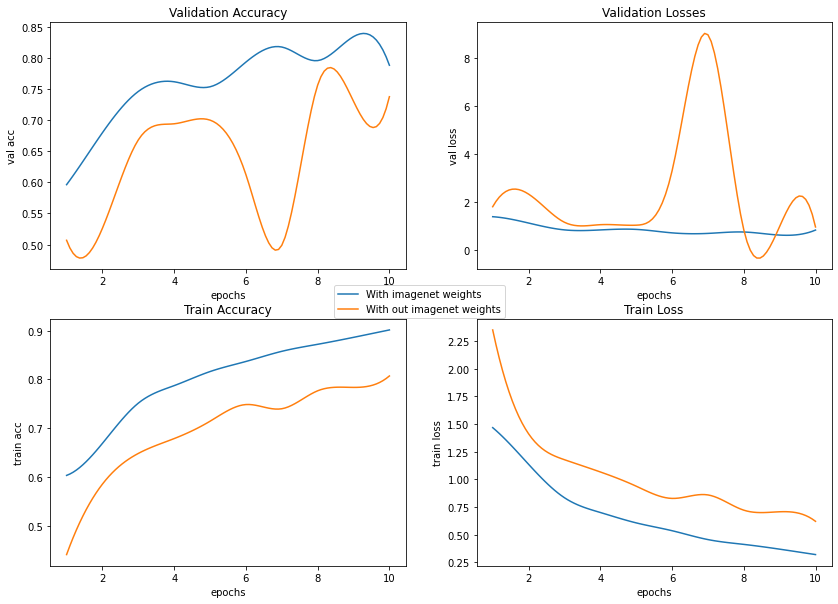
\includegraphics[width=1\columnwidth]{figures/comparison_softmax.png}
        \caption{\label{fig:comparison-softmax} ImageNet vs random performance.}
\end{figure}

\noindent Because of this, we then decided stick to models with ImageNet weights for our further analysis.

\subsubsection{Comparing CNN architectures}
Further, we test the performance of several CNNs. As mentioned in \hyperref[subsec:cnn]{CNN architecture}, we do not want too many parameters so we could still train them locally. We tested all architectures for 10-15 epochs. \\

\noindent These were the results:

\begin{table}[ht]
\begin{tabular}{ c c c c c }
  \hline
    \(Architectures\) &  \(ACC_{10}\) & \(s/epoch\) & \(ACC_{10}\)/time \\ \hline \hline
  ResNet50  & 81,9 & 532 & 0.15 \\ \hline
  ResNet50V2  & 85,4\% & 411 & 0.21 \\ \hline
  DenseNet100  & 89,7\% & 506 & 0.18\\ \hline
  InceptionNetV3  & 90\% & 271 & 0.33\\ \hline
\end{tabular}
\caption{ \(ACC_{10}\) denotes the validation accuracy after 10 training epochs. $s=$seconds.}
\end{table}

\noindent We also tried to use several versions of EfficientNet, but sadly our kernel always died pretty quickly. \\

\noindent As you can see, InceptionNetV3 had - compared to the others - an outstanding performance considering training time. This is why we selected it to be the model, which we will train further and of which we will recycle the weights later for the Siamese Model Training. \\

\noindent We then decided to train for 70 epochs in total and evaluate the best model checkpoint with the best validation accuracy on our test dataset. We achieved an test accuracy of $94.45\%$ and a k3-accuracy of $98.79\%$ on our test data, which was quite impressive. \\
We then analyzed the accuracy for every species and found that as one might expect, the model was really good at recognizing species with many images, while struggling with the uncommon ones. \\
For example, it completely failed to detect the least common species ("Frasier Dolphins" with only 14 images). Strangely, the best performing species were the "Commersons Dolphins", with only 90 images in the database. We assume this has to do with the unique, black and white look of their dorsal fins and the very high image quality of the images, which you can see \href{https://drive.google.com/uc?id=1R8KGr8MjN4bOIDqaMQZQiSRsMcOiiZEd}{here}.

\section{Our Triplet Loss Model}
\addcontentsline{toc}{section}{Our Triplet Loss Model}
\label{sec:triplet_loss_model}

\subsection{Specific Dataset}
Since the \hyperref[sec:kagglechallenge]{Kaggle Challenge} already provides a testing mechanism, we only had to choose a validation dataset. We already disregarded more then half of individuals by now so we do not want to throw away more data. Hence, we decided to only consider individuals with $>3$ images. We then used a method very similar to the smart \hyperref[subsubsec:smart-batches]{Smart Batches Algorithm}:

\begin{enumerate}
    \item Iterate over all the individuals with $>3$ images.
    \item Take the first two images and put them to the side to make sure we don't disregard individuals.
    \item Shuffle the remaining images (with a seed).
    \item According to the split ratio $S$ (we choose $0.1$), take the first $\lceil S * len(remaining\  images) \rceil$ individuals as your validation dataset.
    \item Use all the other images as the train dataset.
\end{enumerate}

\noindent Then we called the \hyperref[subsubsec:smart-batches]{Smart Batches Algorithm} and do the remaining standard preprocessing steps. We used the seed $0$.

\subsection{Configurations and Hyperparameters}
To test our hypotheses we  will train these models:
\begin{enumerate}
    \item InceptionV3 Model with the weights pretrained on the Softmax species.
    \item InceptionV3 with imagenet weights.
    \item Resnet50V2 with imagenet weights.
\end{enumerate}

\noindent For simplicity, we will refer to the models from now on as "Species-Weights", "ImageNet-Weights" and "Control-Model". \\
As for the embedding block, which we put on top of the CNN, we choose this architecture: 3 Dense-Layers with $512$, $256$ and $256$ output neurons respectively and $ReLu$ - activation functions. We then choose to use a l2-normalizing layer as our final output layer to enforce more evenly distributed distances to then later be able to better identify new individuals. \\
We do automated online semi hard triplet mining with a default margin of $1$.


\subsection{Evaluation}
\subsubsection{Procedure}
\noindent Since the the \hyperref[sec:kagglechallenge]{Kaggle Challenge} offers a nice automatic way of testing models, we had to only come up with a validation procedure for our inter-model comparison. We decided for this 2 stage validation procedure:




\noindent Firstly since our model should learn to recognize individuals it has seen before, we decided to measure the accuracy
of the images of the known individuals being correctly matched, as well as the k5-individual accuracy and the accuracy of classifying the right species. To achieve this we firstly we calculated the embeddings of our train and validation datasets. Then we computed the pairwise distance matrix with an euclidean metric of the two embeddings and sort out the labels with the 5 closest values. With these labels we now could calculate the beforehand mentioned accuracies. In addition we used \href{https://umap-learn.readthedocs.io/en/latest/basic_usage.html}{UMAP} to visualize a dimensional representation of our embeddings. 

\noindent Secondly our model should also recognize when it has not seen an individual before. For that we used the individuals with only one picture and calculated there embeddings. We then calculate the pairwise distance matrix of those embeddings with the train embeddings and sorted out the distance to the nearest neighbor. We then compared this distance to with the average distance of individuals which our model is already familiar with. For that we created density plots of the distributions.

\subsubsection{Analysing General Training Behaviour}

\begin{figure}[ht] 
        \centering 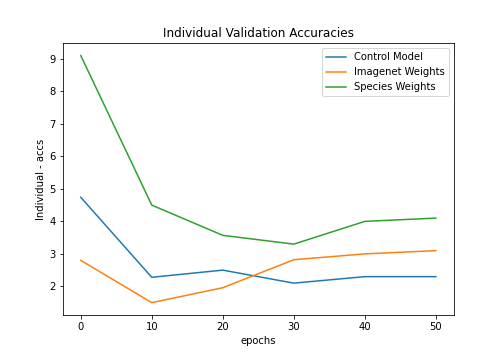
\includegraphics[width=1\columnwidth]{figures/sieamesevalacc.png}
        \caption{\label{fig:sialoss} Individual Validation Accuracies}
\end{figure} \noindent 
When looking at these results in Figure 7 we were really confused at first. Why does every Model has it's best performance before training? Therefore we did some data analysis:

\noindent Before training all the weights of our embedding block are randomly initiated. Thus a high Validation Acuraccies arises probably from the very uneven distribution of individual counts. First we have to look at the dataset which we use for our siamese model training and validation, the dataset containing all the individuals with at least 2 images. The top 300 individual of this data, make out 5\% of the individuals and 40\% of the images. So if we know choose to random images from the data the chances of getting the same individual are quite high.
Even more interesting is to which species these most 300 common individuals belong to:
\begin{figure}[ht] 
        \centering 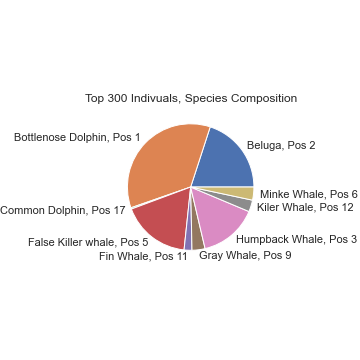
\includegraphics[width=1\columnwidth]{figures/compo.png}
        \caption{\label{fig:compo} Species Composition of top 300 Indivuals. \textit{Pos} refers to the degree of frequency}
\end{figure}\\
We can clearly see, that these top 300 individuals belong mainly to the most frequent classes. In addition what is very interesting is that the species accuracy, the likelihood of the next neighbor in the embedding space being of the same space, is for all models around around 80\% after epoch 30. If we combine these two facts, we can refer that the most frequent classes are quite densely packed together in the embedding space. Therefore the images of the 300 most common individuals, which make out a huge part of our training data, are also most likely in those densely packed embedding spheres. We assume that therefore we have a lot "Hard-Triplet-Pairs" in within these spheres of the most frequent species. And since we are training on "Semi-Hard-Triplets" our theory now is, that initial accuracy of our model decreases, because it arises from correctly matching the most frequent individuals, which our model is then not training to do.
In addition the 2d UMAP-plots of our embeddings support these hypothesis.

\subsubsection{Species Weights vs Imagenet Weights}
All the 3 validation accuracies (Individual, k5-Individual, Species) and also the 2d-UMAP-plots before and while training show that the Species Weights Model performs significantly compared to the Imagenet-Model.


\subsubsection{Species Weights vs Imagenet Weights}
All the 3 validation accuracies (Individual, k5-Individual, Species) and also the 2d-UMAP-plots before and while training show that the Species Weights Model performs significantly compared to the Imagenet-Model.

\subsubsection{Imagenet Weights vs Control Model}
Although the InceptionV3 Model outperforms the Resnet50V2 model in terms Individual and k5 accuracy the effect is by far not as strong in the Softmax case. Especially if we into account that it took the InceptionV3 model almost double as long as the Control Model to have a convergent training loss. 

\subsection{Kaggle Test Dataset Evaluation}
Since our best performing model is quite ironically the Species-Model before training even one epoch with the triplet loss, we choose it for the test evaluation. 
To now test our model we had to create a submission.csv according to \href{https://www.kaggle.com/competitions/happy-whale-and-dolphin/overview/evaluation}{this guidelines}.
Most importantly is that we not only have to identify individuals which we have seen before, but also new individuals. 
For that we used the \href{https://drive.google.com/uc?id=1syxxE7cTRHr7iRN7vo19Wp3ewCINJxEg}{density plot} of the average distance of new individuals to the their next neighbors compared to known individuals. Looking at the distributions we decided to expect there to be a new individual at a distance of $0.35$. 
To generate the submission.csv we now first had to compute the embeddings of all our data (the Kaggle training data) and the embeddings of the Kaggle test data. Then we computed the pairwise distance matrix and sorted out the 5 closest neighbors and their corresponding labels. For every test image we know iterated through the list of the 5 closest neighbors. If the distance to the neighbor was bigger then $0.35$ we inserted "new\_individual" into the list at that position. Like this we achieved a score of $0.077$.

\section{Conclusion}
\addcontentsline{toc}{section}{Conclusion}

\subsection{Hypothesis 1}
Is a ”lazy” approach of just using prebuild \& pretrained architectures and preconfigured loss functions sufficient enough to produce significant results in individual classification?
\\
With a final Kaggle Evaluation Score of $0.077$, our model did really not achieve sufficient result to be use full in anyway in marine nature conservation. Therefore we assume that a similar approach is most likely also nut sufficient enough for other domains of nature conservation.

\subsection{Hypothesis 2}
Is Softmax classification training success a useful indicator for triplet loss training success? To be specific: Does the best performing CNN architecture under Softmax also show best performance of under triplet loss?
\\
With InceptionV3 model with imagenet weights just barely outperforming the Resnet50V2 model with imagenet weights in regard of validation accuracy, we do not have enough data to either support or deny this hypothesis.

\subsection{Hypothesis 3}
Can you reduce triplet loss training time with network weights pretrained on Softmax classification?
\\
Because of the strong performance of our InceptionV3 Model pretrained on classifying the whale and dolphins species compared to the other models, we have strong reason to believe this hypothesis.



%----------------------------------------------------------------------------------------
%	REFERENCE LIST
%----------------------------------------------------------------------------------------
\phantomsection
\bibliographystyle{apacite}
\bibliography{sources}

%----------------------------------------------------------------------------------------
%	ACRONYM LIST
%----------------------------------------------------------------------------------------
\begin{acronym}
% Add your Acronyms here and be careful to always use them in the text!
% See examples in example.tex
\end{acronym}

%----------------------------------------------------------------------------------------
%   END DOCUMENT
%----------------------------------------------------------------------------------------
\end{document}